\section{Cracker Shops}
\label{sec:g-cracker-shops}
\problemlink{https://www.codechef.com/problems/ACM14KG1}{CodeChef ACM14KG1}
\source{ICPC 2014--15 Kharagpur Online Re-contest (PYQ, ACM14KG1)}{Medium--Hard}

\problemstatement{Shops $1..N$ each sell a set of cracker types from $1..M$
(all $M$ types appear somewhere). For every shop $i$ find $j\le i\le k$ such
that shops $j..k$ together sell all $M$ types, minimising $k-j$ and then $j$.
($\sum N,\sum M,\sum X\le5\cdot10^5$.)}

\begin{patternbox}
Two layers: \textbf{two pointers} give, for each left end $j$, the shortest
covering window $[j,e_j]$; then every query window is one of these, possibly
\emph{stretched} to reach $i$. Monotone boundaries $\Rightarrow$ a sliding
ordered set.
\end{patternbox}

\subsection*{Approach and intuition}

\textbf{Step 1.} For each $j$ let $e_j$ be the smallest $k$ such that
$[j,k]$ covers all types ($\infty$ if none). As $j$ grows, $e_j$ never
decreases, so a standard two-pointer sweep with a counter per type computes
all $e_j$ in linear time.

\textbf{Step 2.} For shop $i$ and a left end $j\le i$, the best window starting
at $j$ that contains $i$ is $[j,\max(e_j,i)]$. Split the candidates:
\begin{itemize}
  \item $e_j<i$: the window is $[j,i]$, length $i-j$, best for the
        \emph{largest} such $j$. Because $e$ is non-decreasing, these $j$ form a
        prefix $1..p-1$, so the candidate is $j=p-1$.
  \item $e_j\ge i$: the window is $[j,e_j]$, scored by $(e_j-j,\,j)$. These
        $j$ lie in $[p,i]$ --- a range whose both ends only move right as $i$
        grows. Keep them in an ordered set and read its minimum.
\end{itemize}

\begin{center}
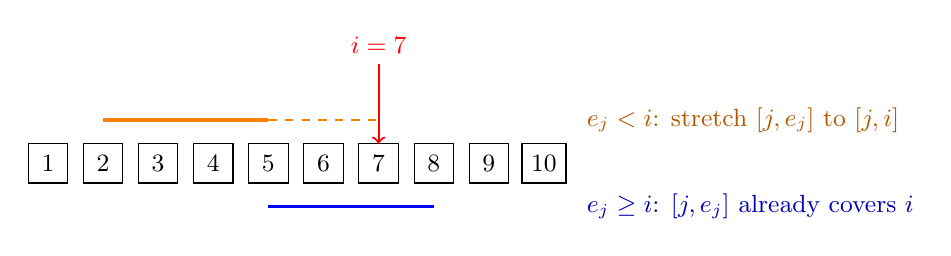
\begin{tikzpicture}[x=0.7cm,y=0.55cm]
  \foreach \x in {1,...,10} \node[draw,minimum size=0.5cm] at (\x,0) {\small\x};
  \draw[very thick,orange] (2,1) -- (5,1);
  \draw[orange,dashed,thick] (5,1) -- (7,1);
  \node[anchor=west,orange!70!black] at (10.6,1) {\small $e_j<i$: stretch $[j,e_j]$ to $[j,i]$};
  \draw[very thick,blue] (5,-1) -- (8,-1);
  \node[anchor=west,blue!70!black] at (10.6,-1) {\small $e_j\ge i$: $[j,e_j]$ already covers $i$};
  \draw[->,red,thick] (7,2.3) node[above] {\small $i=7$} -- (7,0.45);
\end{tikzpicture}
\end{center}

\subsection*{Algorithm}
\begin{algorithmic}[1]
\State compute $e_j$ by two pointers
\State $open\gets\emptyset$ (pairs $(e_j-j,j)$), $p\gets1$
\For{$i=1$ \textbf{to} $N$}
  \State \textbf{if} $e_i<\infty$: insert $(e_i-i,i)$
  \While{$p\le i$ \textbf{and} $e_p<i$} erase $(e_p-p,p)$; $p\gets p+1$ \EndWhile
  \State $best\gets\min(open)$ as window $[j,e_j]$
  \State \textbf{if} $p>1$: compare with window $[p-1,i]$ (length $i-p+1$, tie on smaller $j$)
  \State print $best$
\EndFor
\end{algorithmic}

\dryrun{Test 2: shops $\{1\},\{2,3\},\{1\}$, $M=3$. $e_1=2$, $e_2=3$,
$e_3=\infty$. $i=1$: open $=\{(1,1)\}\Rightarrow(1,2)$. $i=2$: open
$\{(1,1),(1,2)\}$, tie on length, smaller $j$ $\Rightarrow(1,2)$. $i=3$:
$e_1=2<3$ so $j=1$ leaves, $p=2$; open $\{(1,2)\}\Rightarrow[2,3]$; the
stretched candidate $[1,3]$ has length $2>1$. Output $1\,2$, $1\,2$, $2\,3$.
\checkmark}

\subsection*{C++17 implementation}
\cppfile{greedy/25_cracker_shops.cpp}

\begin{complexitybox}
\textbf{Time:} $O((N+\sum X)+N\log N)$. \textbf{Space:} $O(N+M+\sum X)$.
\end{complexitybox}

\begin{pitfallbox}
\begin{itemize}
  \item The editorial's ``corner case'': near the end every minimal window
        ends before $i$, so the answer is a \emph{stretched} window --- the
        $j=p-1$ candidate.
  \item Ties: minimise length first, then $j$.
  \item Up to $10^4$ tests: allocate per test only $O(N+M)$ memory, never
        a global array of fixed maximum size reset each time.
\end{itemize}
\end{pitfallbox}
